\chapter{Weyl semimetals}

\section{Physical aspects}


\section{Topological description}\label{sec:semimetal-topology}

%TODO introductory paragraph

\subsection{3D Chern insulators}

To get a good intuition for the topological description of Weyl semimetals, it is useful to first consider a fully insulating material with similar properties. Suppose we have a three-dimensional material that is not subject to any additional symmetries. Such a material is called a 3D Chern insulator, in analogy to the 2D Chern insulator studied in Section \ref{sec:Chern}.%TODO
This system is not a semimetal in the sense that there are no band crossings in the bulk; still, in many respects it can be considered a limiting case of a Weyl semimetal, where the number of Weyl points is zero. %TODO figure out acceptable wording

From the Atland--Zirnbauer classification in Table \red{[reference]},%TODO
one might expect a 3D Chern insulator to be topologically trivial. However, as seen before in equation \red{[reference] (and perhaps also in 3D BHZ/Kane--Mele if I discuss this in ch. 2)},%TODO
the full topological classification of materials depends not only on the top-dimensional topology, but also on that borrowed from lower-dimensional subspaces. In the case of a 3D Chern insulator, this topology arises on two-dimensional slices of the Brillouin zone; an example of such a slice is highlighted in Figure \ref{fig:3D_Chern_insulator}.
\begin{figure}[htb!]
	\centering
	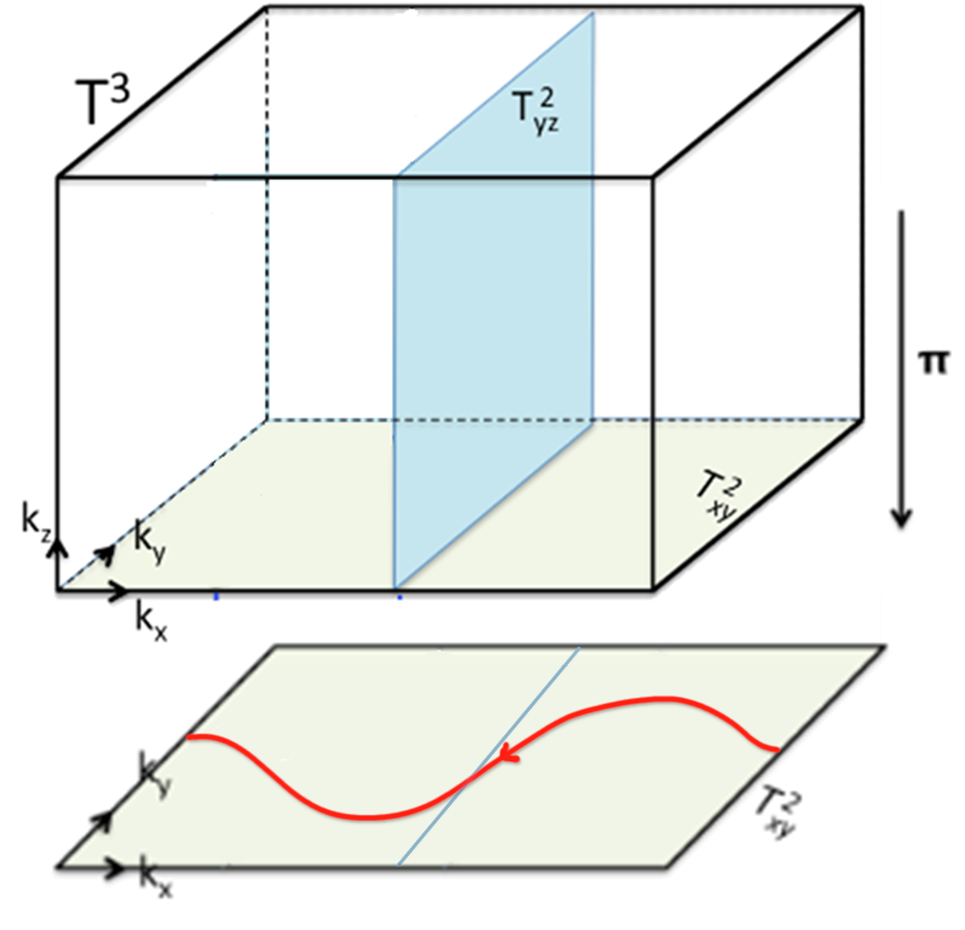
\includegraphics[width=.5\linewidth]{Images/3D_Chern_insulator}
	\caption{
		\red{[Temporary figure]} %TODO fix
		Three-dimensional Brillouin torus $\T^3$ of a Chern insulator, with a two-dimensional slice $\T_{yz}^2$ indicated in blue. A projection onto a surface Brillouin zone in the $xy$-direction is also shown, with an example Fermi loop of gapless states in red. In this example, the slice $\T_{yz}^2$ has a Chern number of $C_{x} = 1$. Hence, its projection onto the surface is a 1D loop that features one band crossing.
		Figure adapted from \cite{Mathai_math-review}.}
	\label{fig:3D_Chern_insulator}
\end{figure}

There are three topologically distinct ways to slice up the three-torus, all perpendicular to one of the three coordinate directions.\footnote{
	Other 2D slices exist, such as those going diagonally across, but these can all be considered linear combinations of the three ``orthogonal'' slices. To be precise, the different classes of 2D subspaces of $\T^3$ form the second homology group $H_2(\T^3)\cong\Z^3$, and this group is \emph{generated} by the orthogonal slices.}
These slices have the topology of a two-torus $\T^2$, and a Chern number can be obtained by integrating the Berry curvature $\Fc$ of the system over them: for example, perpendicular to the $x$ direction there is a Chern number $C_{x} = \int_{\T_{yz}^2}\mathcal{F}$.\footnote{
	Note that it does not matter where along the Brillouin zone this $yz$-slice is taken: the Chern number is an integer, while the system is continuous. This means the $x$ coordinate can be changed continuously without changing the resulting Chern number.}
This results in a classification by three distinct Chern numbers $C_x$, $C_y$ and $C_z$, and in the literature (e.g. \cites{Vanderbilt_2018}{Liu_photonic-Chern-vector}) these are commonly arranged in a so-called \emph{Chern vector}
\[
	\vb{C} = \begin{pmatrix}
		C_x \\ C_y \\ C_z
	\end{pmatrix} \in \Z^3.
\]

Importantly, these three Chern numbers are all induced by a single two-form $\Fc$. In this sense, there is an exact correspondence between topologically distinct Berry curvatures $\Fc$ and Chern vectors $\vb{C}\in\Z^3$. This is precisely what motivates the use of cohomology for classification: just like in the 2D Chern insulator, the two-form $\Fc$ can be considered to represent a class in the second cohomology group,
\begin{equation}\label{eq:2nd-cohom-t3}
	[\Fc]\in H^2(\T^3)\cong\Z^3. 
\end{equation}
As a result, this group precisely classifies the distinct topological phases of the system.\footnote{
	More fundamentally, a complex vector bundle called the \emph{valence bundle} can be associated to a gapped Hamiltonian, and the second cohomology group classifies the different complex vector bundles over a manifold.}

\subsubsection{Boundary states}

Before moving on to a system with Weyl points, it will be instructive to study the gapless modes that arise on the surface of a 3D Chern insulator with non-zero Chern vector. Figure \ref{fig:3D_Chern_insulator} illustrates the case where $\vb{C} = (1,0,0)\tran$. In this case, $\T_{yz}^2$ is the only orthogonal slice with a non-zero Chern number, and as such the material lattice can be thought of as a stack of 2D Chern insulators spanning the $y$ and $z$ directions, stacked together in the $x$ direction. $\T_{yz}^2$ can effectively be considered the Brillouin zone of such a 2D Chern insulator.

Recall from our discussion in Section \ref{sec:Chern} that a 2D Chern insulator with a Chern number of 1 has a single chiral edge mode, which manifests as a gapless state on the one-dimensional surface Brillouin zone. %TODO Extra canceling edge modes may appear <=> folding of the Fermi loop
This logic can be translated to the the three-dimensional case, where such slices are stacked in the $x$ direction. Suppose there is a projection $\pi$ along the $z$ direction, onto a two-dimensional surface Brillouin zone $\ext{\T}_{xy}^2$. Then the two-dimensional slices $\T_{yz}^2$ project down to a one-dimensional loop $\pi(\T_{yz}^2)\cong S^1$ containing a single point-like gapless state. As the $\T_{yz}^2$ slice is moved around in the $x$ direction, this band crossing point moves continuously along the $y$ direction, by continuity of the Hamiltonian. It follows that the full two-dimensional surface Brillouin zone must contain a loop of gapless states going across the $x$ direction, as depicted in the figure. This loop is called a Fermi loop, in analogy with the Fermi arcs in a Weyl semimetal, and the existence of such loops is experimentally well documented \red{[references]}. %TODO refs
Moreover, the chirality of the edge modes can be used to assign a consistent orientation to this loop. %TODO note about linked loops, extra topology etc.

Fermi loops admit a natural topological description in terms of homology. Being oriented loops, they precisely represent a class in the first homology group $H_1(\ext{\T}^2)$ of the surface Brillouin zone. Furthermore, it is possible to define an oriented \emph{Dirac loop} \red{[I don't know if there is an established term for this]} %TODO terminology
$\ell$ in the bulk Brillouin zone in such a way that its projection $\pi(\ell)$ onto the surface in any direction is exactly the Fermi loop. This loop $\ell$ is not a gapless feature \red{[it does seem to be related to gauge singularities, at least in WSMs]}, %TODO
but it is rather interesting topologically: it represents a first homology class in the bulk Brillouin zone,
\[
	[\ell]\in H_1(\T^3)\cong\Z^3.
\]

It is not a coincidence that this first homology group is isomorphic to the second cohomology group $H^2(\T^3)$ from Equation \eqref{eq:2nd-cohom-t3}. This equivalence is a result of \emph{Poincar\'e duality}, which is the statement that for any closed oriented $d$-dimensional manifold $M$, the isomorphism
\[
	H_n(M) \cong H^{d-n}(M)
\]
holds for any integer $n$. In the present case, this duality can be stated intuitively in terms of Chern numbers, which count the number of signed intersections of the Dirac loop with the different two-dimensional slices of the Brillouin zone. This duality can be summarised schematically as follows:
\begin{equation}\label{eq:duality-scheme}
	H^2(\T^3) \ni [\Fc] \overset{\rm integration}{\iff} %TODO change "integration"?
	\vb{C} \overset{\rm intersections}{\iff} [\ell] \in H_1(\T^3).
\end{equation}
This Poincar\'e duality ensures that the classifications in terms of first homology and second cohomology are completely equivalent in this case. Importantly, however, Poincar\'e duality depends on orientability, and it will not hold when we consider non-orientable Brillouin zones in the next chapter. As such, the question of which group provides the right classification of such a system will be key. For the moment, we turn our attention to the topology of Weyl points in the simpler orientable setting.


\subsection{Introducing Weyl points}

Consider a Weyl semimetal with a set of $k$ Weyl points
\[
	W \equiv \set{w_1,w_2,\ldots,w_k}\subset \T^3.
\]
Then the charge of a Weyl point $w_i$ is given by the Chern number
\begin{equation}
	C_w = \int_{S_w^2}\!\Fc,
\end{equation}
where $S_w^2$ is a sufficiently small 2-sphere centred at $w$---in particular, it must be small enough to contain no other Weyl points in its interior. Naively, this might lead us to expect that a semimetal phase is classified by the second cohomology group of the collection of all these spheres:
\begin{equation}\label{eq:2nd-cohom-spheres}
	H^2\left(\bigcup_{i=1}^k S_{w_i}^2\right)\cong \bigoplus_{i=1}^k H^2(S_{w_i}^2) \cong \Z^k.
\end{equation}
However, this classification runs into two problems: it ignores the global cancellation of charge, and it also ignores the additional topology on two-dimensional slices discussed in the previous subsection. Both of these issues are due to the fact that this group only captures the \emph{local} topology near each Weyl point, and they can be addressed by studying how the different Chern numbers on the Brillouin zone must relate to each other \emph{globally}.

The Nielsen--Ninomiya charge cancellation theorem is one such global relation. It is the statement that all the Chern numbers on these 2-spheres must add to zero:
\begin{equation}
	\sum_{i=1}^{k}C_{w_i} = 0.
\end{equation}
This cancellation can be demonstrated using Stokes' theorem. The argument goes as follows: imagine that the interior of each sphere $S_{w_i}^2$ (i.e.\ a small open 3-ball centred at $w_i$) is removed from $\T^3$. The resulting 3-manifold $X$ looks like a 3-torus with $k$ small ball-shaped holes, and its boundary is given by the collection of spheres:
\[
	\partial X = -\bigcup_{i=1}^k S_{w_i}^2,
\]
where the minus sign induces the correct orientation. Then Stokes' theorem gives
\[
	0 = \int_{\partial X} \dd{\Fc} = -\sum_{i=1}^{k}\int_{S_{w_i}^2}\!\!\Fc = -\sum_{i=1}^{k}C_{w_i},
\]
which is precisely the Nielsen--Ninomiya theorem.

A similar argument can also be applied to study what happens to Chern numbers on two-dimensional slices of the Brillouin zone in this context. This argument is illustrated in Figure \ref{fig:Weyl-point-Stokes}.
\begin{figure}[htb!]
	\centering
	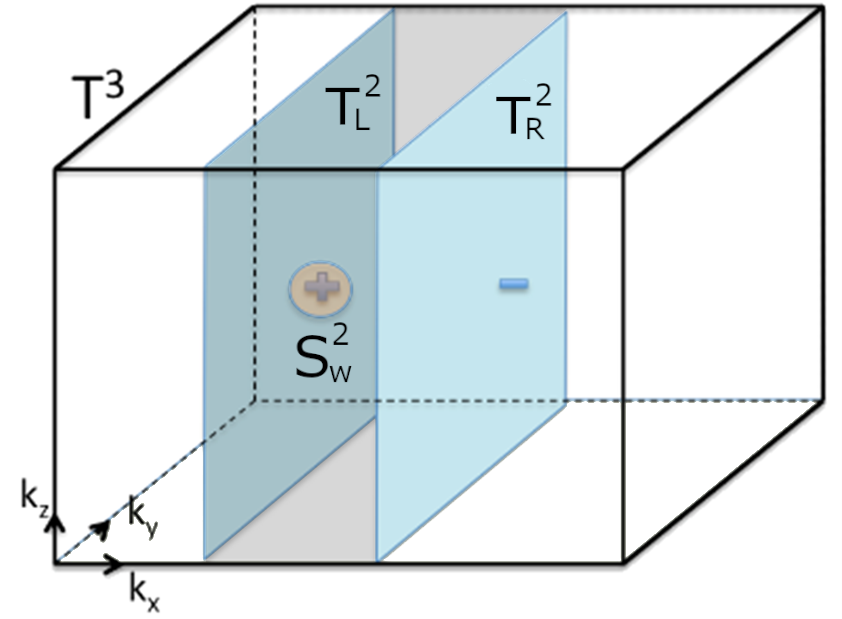
\includegraphics[width=.5\linewidth]{Images/Weyl-point-Stokes}
	\caption{
		Brillouin torus $\T^3$ of a Weyl semimetal with two oppositely charged Weyl points labelled $+$ and $-$. Three two-dimensional subspaces are indicated in blue: a $yz$-like 2-torus on either side of the $+$ point, and a small 2-sphere surrounding it. Given the proper orientation, the blue spaces form the boundary of a three-dimensional manifold $Y$, shaded in grey here.
		Figure from \cite{Mathai_math-review}. \red{[not yet licensed; may need better labelling]}%TODO
	}
	\label{fig:Weyl-point-Stokes}
\end{figure}
Here two slices $\T_L^2$ and $\T_R^2$ are placed on either side of a Weyl point $w$ with charge $C_w = q$, along with a small sphere $S_w^2$ surrounding it. These spaces then bound a three-dimensional manifold $Y$ as indicated in the figure, given the following orientations:
\[
	\partial Y = \T_R^2 - \T_L^2 - S_w^2.
\]
The same Stokes' theorem argument can then be used to relate the Chern numbers $C_L$ and $C_R$ on the respective slices, yielding
\[
	C_R = C_L + C_w = C_L + q.
\]
That is, the Chern number of a two-dimensional slice increases by $q$ every time it passes over a Weyl point with charge $q$. As a sanity check, it should be noted that this process respects the periodicity of the Brillouin torus: when the slice is passed over the entire torus, charge cancellation ensures that the added Chern number is zero in total.

All in all, the presence of Weyl points allows for a finer collection of Chern numbers to appear in the Brillouin zone, beyond the $\Z^3$ Chern vector of the insulating case. This behaviour can be captured using cohomology. The key idea is that the Berry curvature has a singularity at points where the gap closes.\footnote{
	Note that this singularity is required in order for the Chern number to change suddenly when a slice (i.e.\ the integration domain of $\Fc$) is moved over a Weyl point continuously.}
As such, it can only be integrated over subspaces where the gap never closes, so that the set of Weyl points $W$ needs to be excluded. This means $\Fc$ now lives in the second cohomology group of the Brillouin zone minus $W$:
\begin{equation}\label{eq:2nd-cohom-semimetal}
	[\Fc]\in H^2\big(\T^3\setminus W\big) \cong \Z^3\oplus\Z^{k-1},
\end{equation}
where $k$ again is the number of Weyl points. Put differently, classification of semimetallic phases given a set of Weyl points $W$ essentially amounts to classifying the gapped phases on the punctured torus $\T^3\setminus W$.

Notably, this classification addresses both issues present in the $\Z^k$ classification on 2-spheres in Equation \eqref{eq:2nd-cohom-spheres}. Firstly, it incorporates 3D Chern insulator topology in the first term, in the form of the $\Z^3$ from Equation \eqref{eq:2nd-cohom-t3}. Perhaps more subtly, charge cancellation is also incorporated in the form of the reduction by one $\Z$ factor in the second term. This can be understood intuitively: for example, if $k=1$ then the Nielsen--Ninomiya theorem implies that the single Weyl point must have a charge of 0, and so it is not topologically protected. A similar intuition holds for larger $k$, in that the $k$ additional ``degrees of freedom'' which are afforded to the system by the Weyl point charges are reduced by one under the charge cancellation condition. This relation will become more explicit once the Mayer--Vietoris sequence is introduced in Section \ref{sec:Mayer-Vietoris}.

%Notably, there are $k-1$ extra factors of $\Z$ involved in the classification of a Weyl semimetal compared to that of a 3D Chern insulator (cf.\ Equation \eqref{eq:2nd-cohom-t3}). This contrasts with the $k$ factors found for the collection of spheres in Equation \eqref{eqeq:2nd-cohom-spheres}. This reduction by one is a natural result of charge cancellation: for example, if $k=1$ then the Nielsen--Ninomiya theorem implies that the single Weyl point must have a charge of 0, and so it is not topologically protected. A similar intuition holds for general $k\in\N$, in that the $k$ additional ``degrees of freedom'' which are afforded to the system by the Weyl point charges are reduced by one under the charge cancellation condition. This relation will become more explicit once the Mayer--Vietoris sequence is introduced in Section \ref{sec:Mayer-Vietoris}.


\subsubsection{Fermi arcs}

The varying Chern numbers over Weyl points help explain how Fermi arcs arise on the surface. As discussed in the case of a 3D Chern insulator, Fermi loops on the surface arise whenever there is a non-zero Chern number in some direction. Similarly, Fermi arcs begin and terminate whenever the presence of a Weyl point causes a change in the Chern number; this is illustrated in Figure \ref{fig:Fermi-arc-Chern}.
\begin{figure}[htb!]
	\centering
	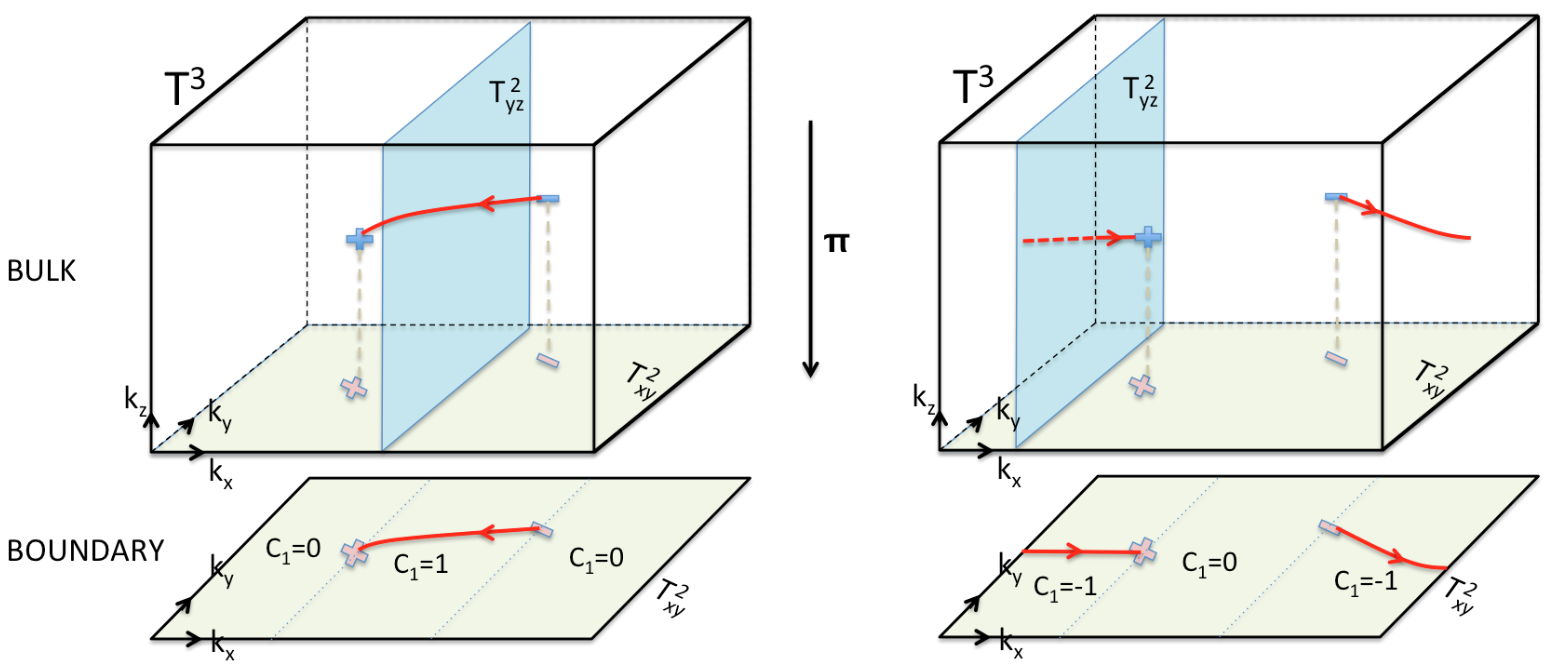
\includegraphics[width=\linewidth]{Images/Fermi-arc-Chern}
	\caption{
		Two semimetal Brillouin zones are shown with the same configuration of Weyl points, but featuring topologically distinct Fermi arcs (shown in red on the boundary). The distinction is due to different bulk Chern numbers: Fermi arcs appear in regions where the bulk Chern number is non-zero. These Fermi arcs can be considered to be the projection of a Dirac string (shown in red in the bulk).
		Figure from \cite{Mathai_math-review}.}
	\label{fig:Fermi-arc-Chern}
\end{figure}

This feature of Weyl semimetals implies they can mediate phase transitions between 3D Chern insulators with different Chern vectors. For example, suppose a pair of Weyl points is created at some point in the Brillouin zone of a trivial insulator ($\vb{C}=0$). These points can then be moved apart in the $z$ direction until they meet again and annihilate at the other end of the torus. In the process, a Fermi arc extends between the projections of the Weyl points on the $xz$ and $yz$-planes, which eventually closes into a Fermi loop. In its final state, the system features a non-zero Chern vector of $\vb{C} = (0,0,1)\tran$. This process was first observed experimentally by Gui-Geng Liu et al.\ in 2022 (see Figure \ref{fig:Weyl-phase-transition}), in the context of a photonic crystal. This was also the first experimental realisation of a 3D Chern insulator \cite{Liu_photonic-Chern-vector}.
\begin{figure}[htb!]
	\centering
	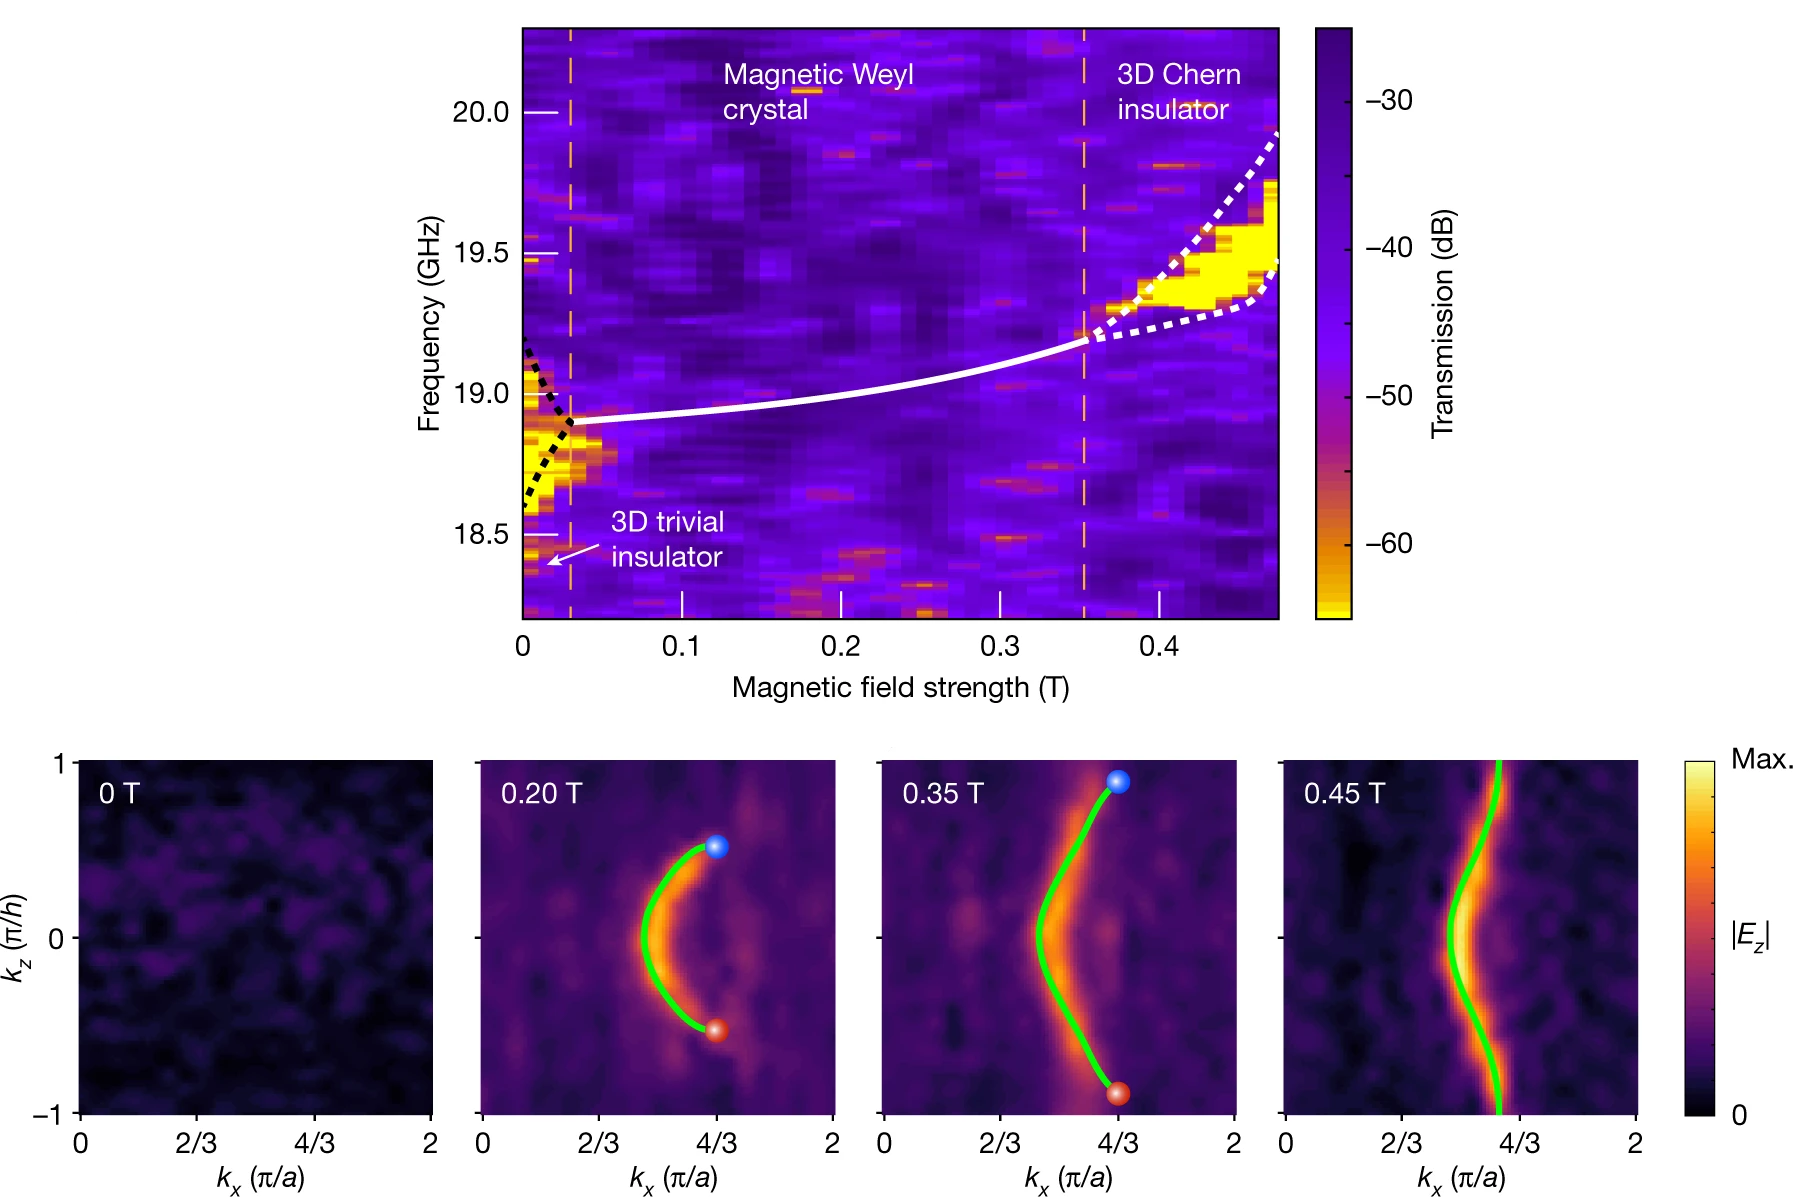
\includegraphics[width=\linewidth]{Images/Weyl-phase-transition}
	\caption{
		\red{[I need to think about how to organise this figure and add a caption]} %TODO
		Figure from \cite{Liu_photonic-Chern-vector}, reproduced with permission from Springer Nature.}
	\label{fig:Weyl-phase-transition}
\end{figure}

Just as Fermi loops can be considered projections of a bulk Dirac loop, so too can Fermi arcs be considered a projection of a bulk \emph{Dirac string}.\footnote{
	A more or less equivalent concept is referred to as \emph{Euler chain} in \cite{Mathai_math-review}, placing the emphasis on topology over physics: ``chain'' here refers the oriented subspaces that homology is founded on.}
Like Dirac loops, these strings can be given an interpretation in terms of homology. The setup is somewhat more subtle in this case: since the Dirac strings have a boundary, they are not loops and as such do not represent homology classes in $H_1(\T^3)$. Instead, they represent classes in the \emph{relative homology group}
\begin{equation}
	H_1\big(\T^3, W\big) \cong \Z^3\oplus\Z^{k-1}
\end{equation}
with respect to the set of Weyl points $W\subset\T^3$. Intuitively, taking the relative homology means that any boundaries lying in the subset $W$ are ignored; for a more precise definition the reader is referred to \parencite[\S 2.1]{Hatcher_algebraic-topology}.

This homology picture provides a classification scheme that is exactly dual to the cohomology classification in Equation \eqref{eq:2nd-cohom-semimetal}; that is, there is an isomorphism
\begin{equation}\label{eq:semimetal-duality}
	H^2\big(\T^3\setminus W\big) \cong H_1\big(\T^3, W\big).
\end{equation}
This is not a direct Poincar\'e duality, but it is nevertheless mathematically rigorous and protected by orientability in the same way.\footnote{
	To be precise, Poincar\'e duality does not hold directly because $\T^3\setminus W$ is not a closed manifold. Instead, for non-compact manifolds $M$ there is a generalized duality $H^n(M)\cong H_{d-n}^{\rm BM}(M)$ where the group on the right is the \emph{Borel--Moore homology}, and this is in turn equivalent to the relative homology in this case. Alternatively, Equation \eqref{eq:semimetal-duality} can be interpreted as a result of the so-called \emph{Lefschetz duality} $H^n(M)\cong H_{d-n}(M, \partial M)$ for manifolds with a boundary.}
The interpretation in terms of Chern numbers given in Equation \eqref{eq:duality-scheme} also still holds here, with the Chern vector and Dirac loops replaced with more general Chern numbers and Dirac strings, respectively.


\subsection{The semimetal Mayer--Vietoris sequence}\label{sec:Mayer-Vietoris}

In the previous section a heuristic Stokes' theorem argument was discussed for charge cancellation on Weyl points. This argument can be generalized by moving to a more abstract cohomology setting, where we are not dependent on the integration of forms; this is important because integration will not be well defined once we move to a non-orientable setting. As an added bonus, the abstract description proves to be richer and provide more detailed information on the possible topological phases for a Weyl semimetal.

The idea is that the relation between the global semimetal topology in Equation \eqref{eq:2nd-cohom-semimetal} and the local charge data in Equation \eqref{eq:2nd-cohom-spheres} can be understood by considering how cohomology classes are mapped between them. That is, one needs to find and study a homomorphism
\begin{equation*}
	\beta: H^2\big(\T^3\setminus W\big) \to H^2\left(\bigcup_{i=1}^k S_{w_i}^2\right).
\end{equation*}
Such a map arises naturally in the context of the \emph{Mayer--Vietoris sequence} for cohomology.

Mayer--Vietoris sequences are used to study how the homology or cohomology of a topological space relates to that of its subspaces. To be precise, let $X$ be a topological space and let $A,B\subset X$ be two subspaces that cover it (i.e.\ $A\cup B = X$). Then there is an \emph{exact sequence} of homomorphisms between cohomology groups,
\begin{equation*}
	\cdots \to H^n(X) \to H^n(A)\oplus H^n(B) \to H^n(A\cup B) \to H^{n+1}(X) \to \cdots,
\end{equation*}
which continues indefinitely in both directions. Exactness means that the image of each map in the sequence is exactly equal to the kernel of the next. In other words, the elements in each term in the sequence which are mapped to zero in the next term are precisely those which ``descend'' from the previous term. In particular, the composition of two subsequent maps always yields zero.

In the context of a Weyl semimetal there is a natural way to divide the Brillouin torus $\T^3$ into two subspaces; this is illustrated in Figure \ref{fig:semimetal-MV}.
\begin{figure}[htb!]
	\centering
	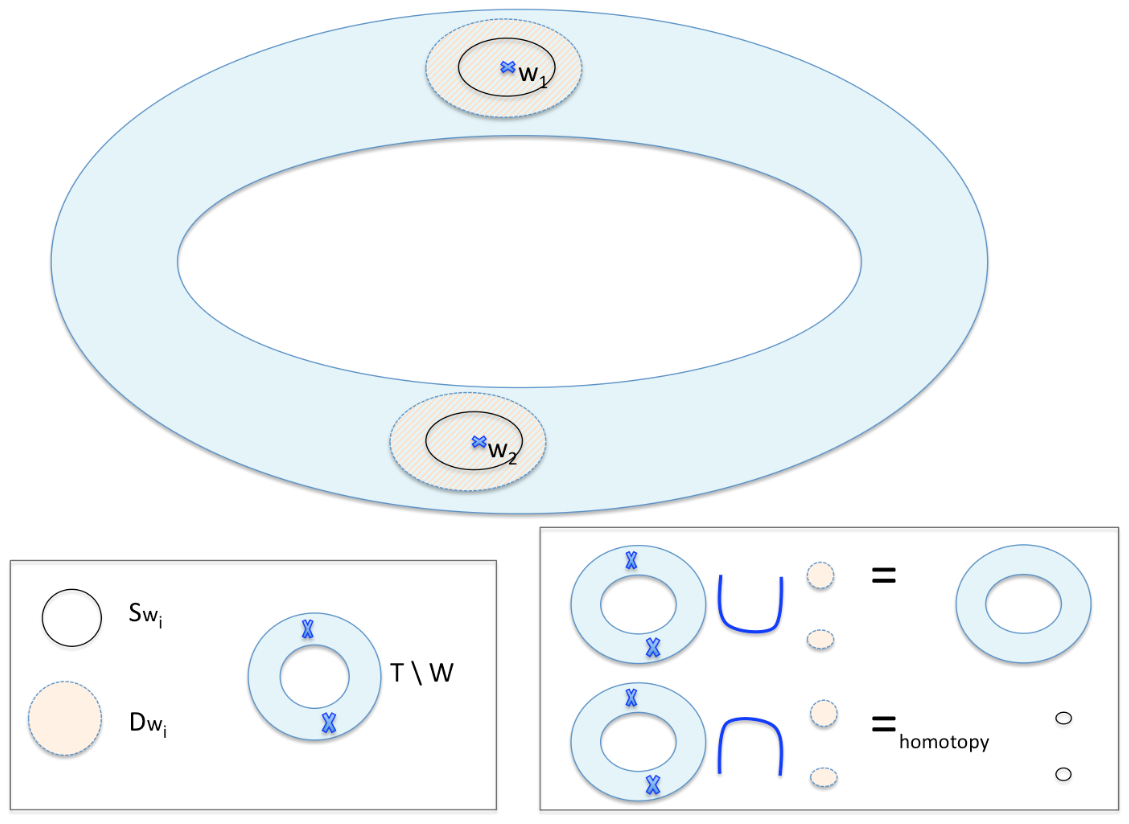
\includegraphics[width=.8\linewidth]{Images/semimetal-MV}
	\caption{
		Schematic two-dimensional representation of the Brillouin torus and the subspaces used to cover it.
		Figure from \cite{Thiang_equivariant}}
	\label{fig:semimetal-MV}
\end{figure}
The first subspace in the covering is the punctured torus $\T^3\setminus W$; we have already encountered this space in classifying topological semimetal phases. The other is the collection $\bigcup_{i=1}^k D_{w_i}^3$ of small open 3-balls centred on the Weyl points $w_i$. The intersection of these two spaces is the same collection of open balls, but each with a single puncture. For our purposes, this intersection has the same topology as the collection of 2-spheres $\bigcup_{i=1}^k S_{w_i}^2$ that we encountered in the context of local Weyl point charges.\footnote{
	To be precise, the punctured 3-balls can be \emph{deformation retracted} into the 2-spheres, making them \emph{homotopy equivalent}. Homotopy equivalent spaces have the same homology and cohomology groups.}
A Mayer--Vietoris sequence can now be written down for these subspaces. The section of this sequence which is relevant to classification is referred to as the \emph{semimetal Mayer--Vietoris sequence}:\footnote{
	Note that the open balls $D_{w_i}^3$ do not appear in this sequence at all. This is because they can be contracted to a point, and hence are topologically trivial in a sense.}
\begin{equation}\label{eq:semimetal-MV-symbolic}
	0\ \to\ \underbrace{H^2(\T^3)}_{\mathclap{\text{3D Chern insulator}}}\ \to\ 
	\underbrace{H^2\big(\T^3\setminus W\big)}_{\text{Semimetal}}\ \overset{\beta}{\to}\ \underbrace{H^2\left(\bigcup_{i=1}^k S_{w_i}^2\right)}_{\text{Local charges}}\ \overset{\Sigma}{\to}\ H^3(\T^3)\ \to\ 0.
\end{equation}
The first three groups in this sequence are already familiar from Equations \eqref{eq:2nd-cohom-t3}, \eqref{eq:2nd-cohom-semimetal} and \eqref{eq:2nd-cohom-spheres} respectively. The last group $H^3(\T^3)\cong\Z$ is represented by volume forms\footnote{
	I.e.\ 3-forms, which are locally proportional to $\dd{k_x}\wedge\dd{k_y}\wedge\dd{k_z}$.}
on the torus; one notable example of such a form is the trivial 3-form
\begin{equation*}
	\dd{\Fc} = 0 \in H^3(\T^3)
\end{equation*}
which appeared in the Stokes' theorem arguments previously. Indeed, the map labelled $\Sigma$ above can be loosely interpreted as the exterior derivative $\dd$. However, a more physically useful interpretation is that $\Sigma$ gives the total charge in the system: it sends a set of Chern numbers on the Weyl points to their sum in $\Z$.

Explicitly, the semimetal Mayer--Vietoris sequence is
\begin{equation}\label{eq:semimetal-MV-explicit}
	0 \to \Z^3 \to \Z^3\oplus\Z^{k-1} \overset{\beta}{\to} \Z^k \overset{\Sigma}{\to} \Z \to 0.
\end{equation}
The exactness of this sequence can be used to extract useful information, especially around the group of local charges $\Z^k$. Here exactness means that $\im(\beta) = \ker(\Sigma)$. This implies that the local charges on the Weyl points sum to zero if and only if they descend from a semimetal. In other words, it implies not only the Nielsen--Ninomiya charge cancellation theorem, but also its converse: any set of Weyl points with charges adding to zero is admissible as a topological Weyl semimetal phase.

In fact, more can be inferred by looking at the maps around the semimetal group $\Z^3\oplus\Z^{k-1}$. Here exactness tells us that $\ker(\beta)\cong\Z^3$. This makes physical sense: if all local charges are zero, the Weyl points are not topologically protected and the system is really in a 3D Chern insulator phase. However, since $\beta$ is a homomorphism, we also find $\beta^{-1}(c)\cong\Z^3$ for a generic charge configuration $c\neq 0\in\Z^k$; that is, every configuration with total charge zero admits a $\Z^3$ worth of topologically different semimetal phases. This makes precise a principle that is also hinted at in Figure \ref{fig:Fermi-arc-Chern}: Weyl semimetals with identical charge configurations may nevertheless be topologically distinct, and their topologies differ by a bulk Chern vector in $\Z^3$.\footnote{
	Properly speaking, the set of topological phases for a given charge configuration is an affine space for $H^2(\T^3)$, since there is no canonical zero Chern vector on a Weyl semimetal. This is worked out in greater mathematical detail in Section 3 of \cite{Mathai_math-review}.}


\subsubsection{The dual homology sequence}

In previous subsections, we have already seen that the cohomology invariants on Chern insulators and Weyl semimetals can be understood equally well in terms of homology groups. As it turns out, this duality can be extended to the semimetal Mayer--Vietoris sequence \eqref{eq:semimetal-MV-symbolic}. The dual of the first two groups was already explored in Equations \eqref{eq:duality-scheme} and \eqref{eq:semimetal-duality}. The latter two groups act on closed manifolds, and so their dual can be obtained from Poincar\'e duality directly:
\begin{equation*}
	H^2\left(\bigcup_{i=1}^k S_{w_i}^2\right) \cong H_0\left(\bigcup_{i=1}^k S_{w_i}^2\right), \qquad
	H^3(\T^3) \cong H_0(\T^3).
\end{equation*}
In both cases, we have a top-dimensional cohomology group (containing volume forms) being dualised to a zeroth homology group, which counts the number of connected components. In particular, since the connected components are the important aspect, the 2-spheres $S_w$ may be substituted for the Weyl points $w$ to simplify:
\begin{equation*}
	H_0\left(\bigcup_{i=1}^k S_{w_i}^2\right) \cong H_0(W).
\end{equation*}
The complete homology dual of \eqref{eq:semimetal-MV-symbolic} is then
\begin{equation}\label{eq:semimetal-homology-sequence}
	0\ \to\ \underbrace{H_1(\T^3)}_{\mathclap{\text{Dirac loops}}}\ \to\ 
	\underbrace{H_1\big(\T^3, W\big)}_{\text{Dirac strings}}\ \overset{\partial}{\to}\ \underbrace{H_0(W)}_{\mathclap{\text{Local charges}}}\ \overset{\Sigma}{\to}\ H_0(\T^3)\ \to\ 0.
\end{equation}

This exact sequence has arisen through taking Poincaré duals of groups in the Mayer--Vietoris sequence, but somewhat miraculously, it continues to be valid even in the absence of Poincaré duality (e.g.\ on a non-orientable manifold). In fact, it can be considered a more fundamental sequence in some ways: it describes the homology of the torus with respect to a single subspace $W$, whereas the Mayer--Vietoris sequence relies on multiple subspaces that cover the torus.\footnote{
	Indeed, this is the first exact sequence introduced in the standard algebraic topology textbooks, e.g.\ in Theorem 2.13 of \cite{Hatcher_algebraic-topology}.}
	
The map indicated by $\partial$ is the boundary map that is used to define homology groups in the first place.\footnote{
	To be precise, homology is defined using boundaries of chains; one can think of the present map as acting on \emph{representatives} of homology classes.}
In this case, it sends classes of oriented Dirac strings in the bulk to the Weyl points that bound them, with a sign given by which end of the string the points are on. For example, for a Weyl semimetal with two Weyl points $W = \set{w_1,w_2}$ connected by a Dirac string $s$, we have $[s]\in H_1(\T^3,W)$ and
\begin{equation*}
	\partial\big([s]\big) = (1, -1)\in H_0(W)\cong\Z^2. 
\end{equation*}
This gives rise to a very natural interpretation of charge cancellation: it automatically follows from the fact that Weyl points on opposite ends of a Dirac string are assigned opposite signs. These opposite charges are then summed to zero by the total charge map $\Sigma$, i.e.\ $\Sigma\circ\partial = 0$. This can also be inferred from the exactness of \eqref{eq:semimetal-homology-sequence}, which additionally tells us that there exists a configuration of Dirac strings compatible with any set of Weyl points with total charge zero.

As emphasised before, this homology sequence encodes exactly the same information as the cohomology Mayer--Vietoris sequence in the simple case where Poincaré duality is preserved. However, once symmetries are imposed on the system, this duality may be broken, and the two sequences become essentially different. In these cases, it becomes necessary to study which of the sequences contains the essential information about the topological phases of the system. As we will review in the next section, the answer is usually that the cohomology sequence needs to be adapted in some way to restore duality and match the information in the more fundamental homology sequence.

\section{Imposing symmetries}\label{sec:T-WSMs}